\section{Application to Color Transfer}
\label{sec-appli-color} 

This section shows how the relaxed and regularized OT formulation can be applied to imaging problems, more specifically to color transfer, and how the regularization and the relaxation improve the results obtained by previous methods. The color transfer problem consists in modifying an input image $X^0$ so that its colors match the colors of another input image $Y^0$. 

\begin{figure*}[h]
\centering
\begin{tabular}{@{}c@{\hspace{1mm}}c@{\hspace{1mm}}c@{}}
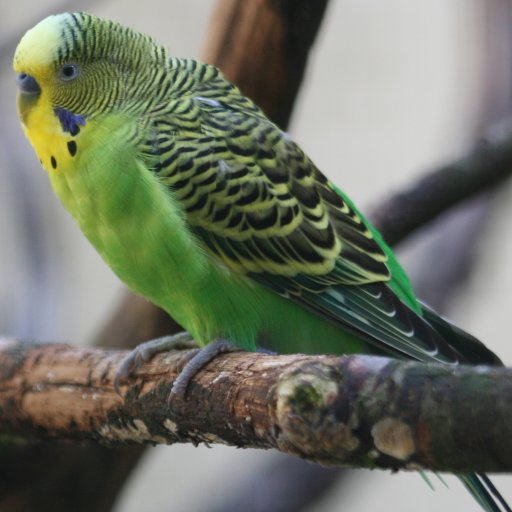
\includegraphics[width=.32\linewidth]{colorization/parrot_1} &
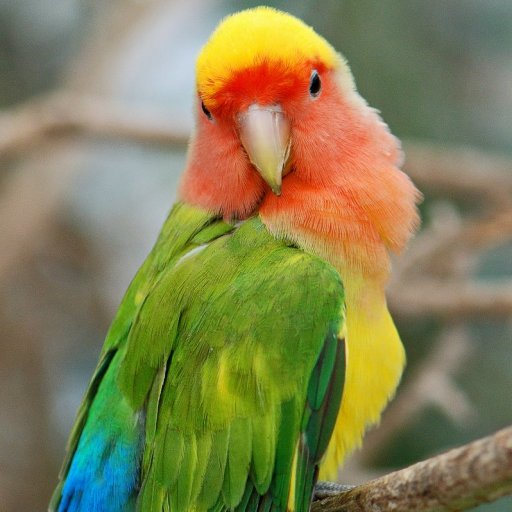
\includegraphics[width=.32\linewidth]{colorization/parrot_2} &
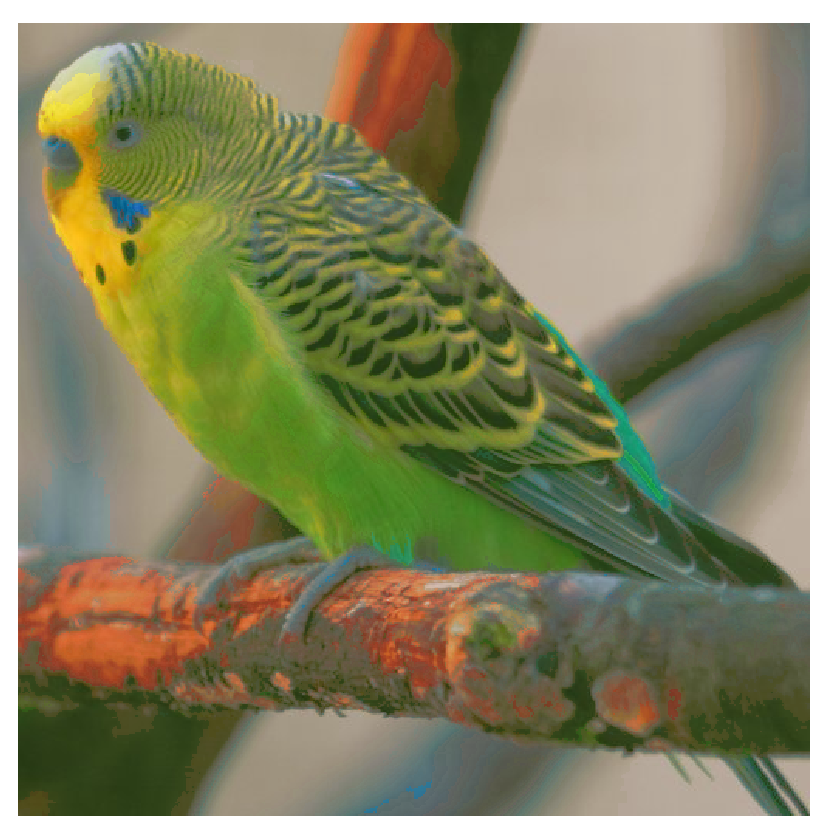
\includegraphics[width=.32\linewidth]{colorization/asymmetricparrot_l00008_KX1_KY1_nn4} \\ 
$X^0$ & $Y^0$ & ${\tilde X^0}$ \\
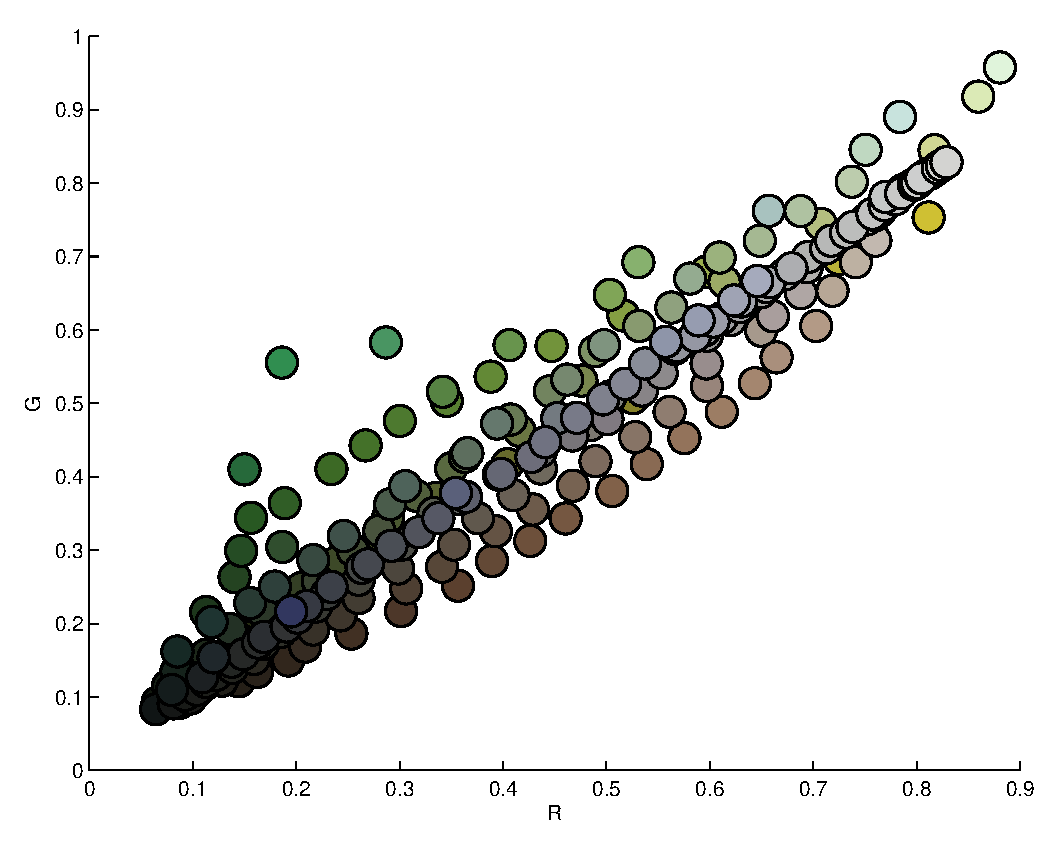
\includegraphics[width=.32\linewidth]{colorization/histo3Dx} &
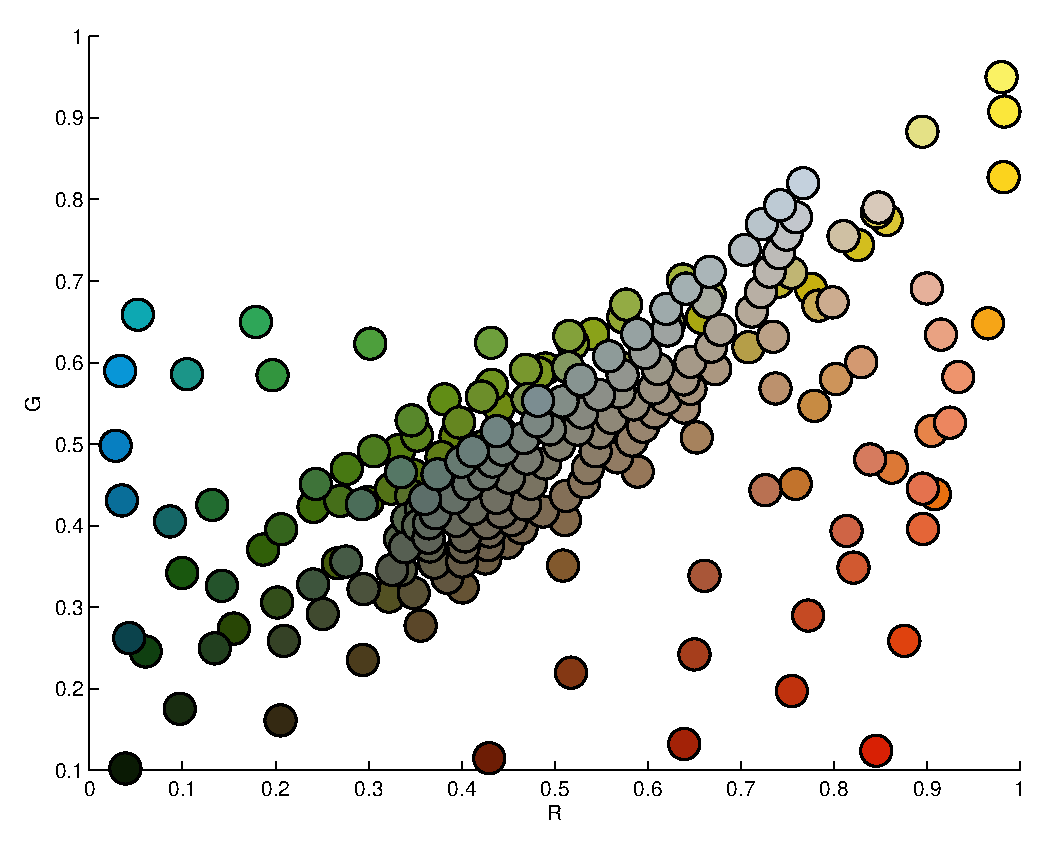
\includegraphics[width=.32\linewidth]{colorization/histo3Dy} &
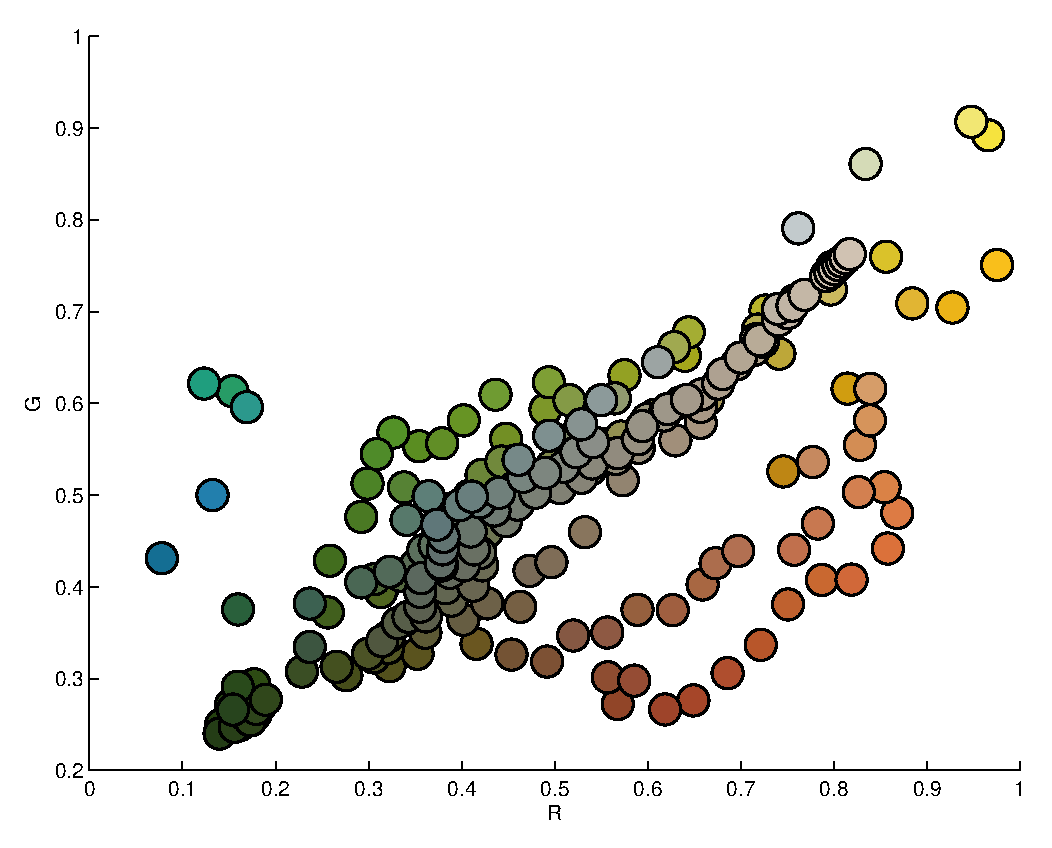
\includegraphics[width=.32\linewidth]{colorization/histo3Du}\\
$\mu_{X^0}$ & $\mu_{Y^0}$ & $\mu_{\tilde X^0}$
\end{tabular}
\caption{Example of the colorization problem. Given images $X^0$ and $Y^0$ with their corresponding 3-D color distributions $\mu_{X^0}$ and $\mu_{Y^0}$ (represented here using their 2-D projection on the RG plane), the goal of colorization methods is to define an image ${\tilde X^0}$ that has the geometry of $X^0$ and a histogram $\mu_{{\tilde X}^0}$  that is similar to $\mu_{Y^0}$.}\label{imcolorization}
\end{figure*}

%%%%%%%%%%%%%%%%%%%%%%%%%%%%%%%%%%%%%%%%%%%%%%%
\subsection{Color Images and Histograms}

In the following, an image is stored as a vector $X^0 \in \RR^{N_0 \times d}$ where $d=3$ is the number of channels (here $d=3$ since we handle color images, with R, G and B color channels) and where $N_0=N_1 N_2$ is the number of pixels ($N_1$ being horizontal and $N_2$ vertical dimensions). The color histogram of such an image $X^0$ can be estimated using the empirical distribution $\mu_{X^0}$. The goal of color transfer algorithms is to compute a transformation $T^0$ such that $(\tilde X^0)_i = T^0(X^0_i)$, where the new empirical distribution $\mu_{\tilde X^0}$ is close (or equal) to $\mu_{Y^0}$. Figure~\ref{imcolorization} shows an example where $X^0$, $Y^0$ are the original input images, the second row displays the 2-D projection of the 3-D distribution of pixels $\mu_{X^0}$ and $\mu_{Y^0}$, and in the third column, we show the $\mu_{\tilde X^0}$ which is the result of applying $T^0$ to $X^0$, where $T^0$ is computed using the method described below. The associated image ${\tilde X^0}$ has the geometry of $X^0$ and the color palette (3-D histogram) of $Y^0$.



%%%%%%%%%%%%%%%%%%%%%%%%%%%%%%%%%%%%%%%%%%%%%%%
\subsection{Regularized OT Color Transfer}

As exposed in Section~\ref{subsec-ot-imaging}, OT is now routinely used to perform color palette modification, and in particular color transfer. As we illustrate below in the numerical examples, relaxing the mass conservation constraint is crucial in order to better match the modes (i.e. the dominant colors) of each distribution. Regularizing the transport is also important to reduce colorization artifacts.

To make the optimization problem~\eqref{eq-symm-reg-energy} tractable for histograms obtained from large scale images, we apply the method on a sub-sampled point cloud. That is to say, before computing the relaxed and regularized transport, we define two smaller point clouds $X$ and $Y$ from $X^0$ and $Y^0$. These clouds are created such that their respective distributions $\mu_X$ and $\mu_Y$ are close to the two original distributions $\mu_{X^0}$ and $\mu_{Y^0}$. The mapping $T$ between these small clouds is then extended by interpolation to the original clouds. The complete algorithm for regularized OT color transfer between a pair of images $(X^0,Y^0)$ is exposed in Algorithm~\ref{alg-rot}. We now detail each step of the method. 

\begin{algorithm}[ht!]
\caption{Regularized OT Color Transfer}
\label{alg-rot}
% \begin{algorithmic}[1]
\Require Images $X^0,Y^0 \in \RR^{N_0 \times d}$, $\la_X,\la_Y \in \RR^+ $, and $k_X,K_X,k_Y,K_Y \in \RR^+$, where $k_X \le K_X$ and $k_Y \le K_Y$.

\Ensure Image $\tilde X^0 \in \RR^{N_0 \times d}$.
% \Statex
\begin{enumerate}
	\algostep{Histogram down-sample} Compute $X,Y$ from $X^0,Y^0$ respectively \\ using K-means clustering.
	\algostep{Compute Mapping} Compute the optimal $\Sig$ such that  $T(X) = \diag(\Sig \U)^{-1} \Sig Y$ by solving eq.~\eqref{eq-symm-reg-energy} with algorithm~\eqref{eq-frankwolfe-update} or the linear program~\eqref{eq-symm-TV} solving with an interior point algorithm.
	%\algostep{Transport up-sample} Compute $\tilde T^0$ by solving eq.~\eqref{eq-upsample}, where  $T(X) = diag(\Sig \U)^{-1} \Sig Y$.
	\algostep{Obtain high resolution result} Compute $\tilde X^0$ with eq.~\eqref{eq-upsample}.
\end{enumerate}
% \end{algorithmic}
\end{algorithm}


%%%%%%%%
\paragraph{Pixels down-sampling} 

We construct a smaller data set $X \in \RR^{N \times d}$ by clustering the set $X^0$ into $N$ clusters with the K-means algorithm (see~\cite{Lloyd57}).
% and~\cite{Quantization} for its application to image quantization). 
Each cluster corresponds to a point $X_i$ in our smaller data set $X$.  The same procedure is done for $Y^0$ to obtain $Y \in \RR^{N \times d}$.%, and we compute  

%%%%%%%%
\paragraph{Graph and $(G_X,G_Y)$ operator} 

As exposed in Section~\ref{sec:regsymme}, the regularization is defined using gradient operators $(G_X,G_Y)$ on graphs $(\Gg_X,\Gg_Y)$ connecting the points in $X$ and $Y$. Inspired by several recent works on manifold learning (see Section~\ref{subsec-regul-intro}), we use here a $n$-nearest neighbor graph, where $n$ is the number of edges adjacent to each vertex, i.e. $\abs{\enscond{j}{(i,j) \in E_X}} = n$ where $E_X$ is the set of edges of $X$. The weights of the graphs are defined as $w_{i,j}=\norm{X_i - X_j}^{-1}$ (same applies for $Y$), which is consistent with the computation of the directional derivatives. An example of this graph can be observed in Figure~\ref{im:matching}. Note that this graph does not need to be fully connected. 

%%%%%%%%
\paragraph{Transport map computation}

The regularized transport map $T$ between the sub-sampled data $(X,Y)$ is computed as
\eq{
	T(X_i)=\left(\diag(\Sig \U)^{-1}\Sig Y\right)_i \qforq i={1,\ldots,N}
} 
where $\Sig$ is a solution of~\eqref{eq-symm-reg-energy}.

%%%%%%%%
\paragraph{Transport map up-sampling}

The transport map $T$ is extended to the whole space using a nearest neighbor interpolation 
% to every point the transport map of the nearest point in $X$: 
\eql{\label{eq-upsample}
	% (\tilde X^0)_{i} = 
	\foralls x \in \RR^d, \quad
	T^0(x) = T(X_{i(x)}) + x - X_{i(x)}, 
	\qwhereq
	i(x) = \uargmin{1 \leq i \leq N} \norm{ x - X_i }. 
} 
Note that this interpolation scheme contains an additive term $x-X_{i(x)}$. This corresponds to adding back the quantization error (due to the K-means sub-sampling) to the nearest neighbors interpolation, which helps to restore small scale textural details, and improves the visual quality of the result.  Note also that one could use smoother interpolation schemes (for instance linear or natural neighbors) to help reducing the quantization error. These interpolations however require to compute a Delaunay tetrahedrization of the 3-D color space, which leads to a significant computational overhead.  

The resulting transport computed in~\eqref{eq-upsample} can now be  applied to the input image $X^0$ to obtain the new pixel values $(\tilde X^0)_{i} = T^0(X^0_i)$.

\begin{figure}[ht]
\centering
\begin{tabular}{@{}c@{\hspace{1mm}}c}
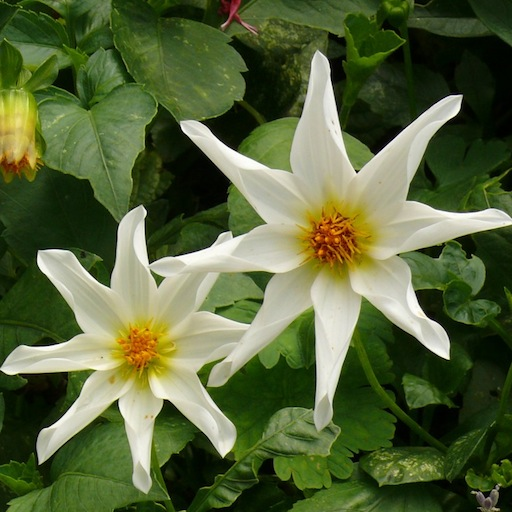
\includegraphics[width=.4\linewidth]{barycenter/flowers/flowers-1.jpg} &
\fbox{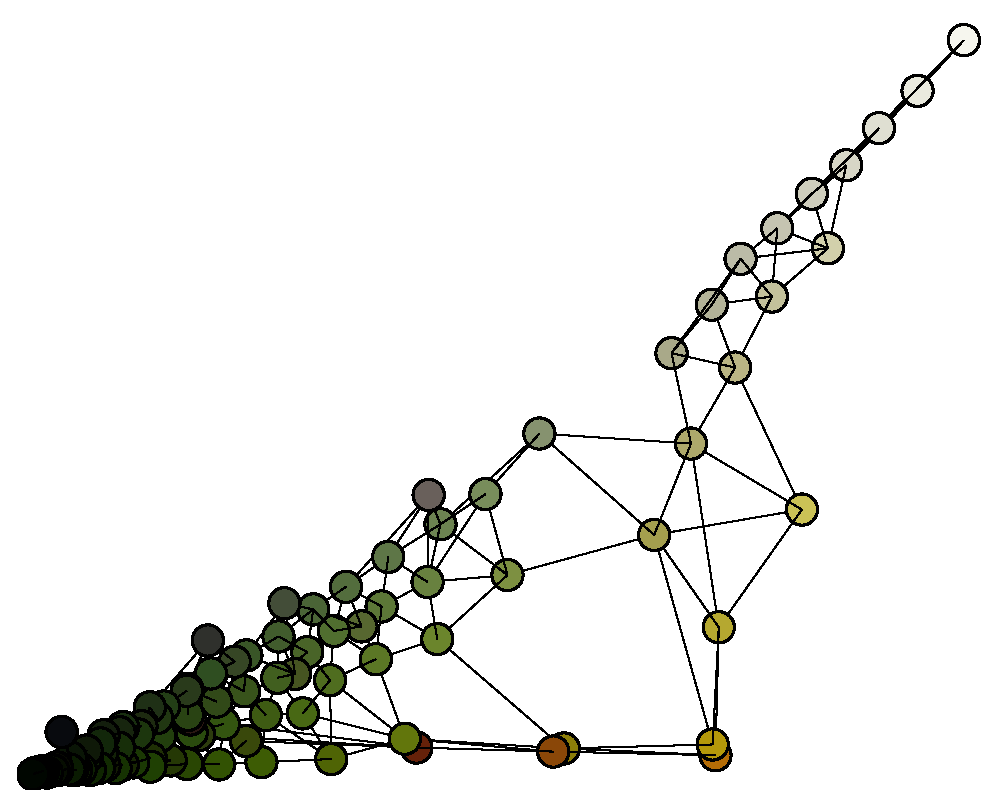
\includegraphics[width=.55\linewidth,height=5.1cm]{coloredgraph}} \\
(a) & (b)\vspace{-0.3cm}
\end{tabular}
\caption{(a) Flower image ; (b) its empirical distribution projected on the Red-Blue plane. The line segments represent the edges $E_X$ of the $n$-nearest neighbor graph computed with $n=4$. \vspace{-0.1cm}}
\label{im:matching}
\end{figure}




%%%%%%%%%%%%%%%%%%%%%%%%%%%%%%%%%%%%%%%%%%%%%%%
\subsection{Parameters Selection}

The color transfer method has several parameters. We explain below their influence and how they were selected in the numerical examples shown in the following section.


%%%%%%%%
\paragraph{Parameters $(p,q)$: Sobolev vs. total variation}

All the numerical results reported in the remaining of the paper are computed using the total variation (TV) regularization, which corresponds to using the parameters $(p,q)=(1,1)$. We found empirically on the color transfer application that both methods produce visually similar results. The main difference is that the resulting optimal $\Sig$ is somehow sparser with the total variation prior, i.e. the resulting weights are more concentrated on a few entries. 


%%%%
\paragraph{Relaxation parameter $\kappa$ } 

The impact of this parameter has already been discussed in Section~\ref{subsec-relaxed-transport}~on synthetic 2-D examples. 

%%%%
\paragraph{Regularization parameters $(\la_X,\la_Y)$} 

%While the impact of these parameters has already been explored in Section~\ref{sec:regsymme} on 2-D examples, we further illustrate it for color transfer of synthetic images.
Figure~\ref{im:synth} shows an example of color transfer between two synthetic images $X^0$ and $Y^0$ shown in Figure~\ref{im:synth}~(a). We apply Algorithm~\ref{alg-rot} to obtain the image ${\tilde X^0}$ with a color palette close to $Y^0$, but with the geometry of the original $X^0$. We now study the influence of the parameters $\la_X$ and $\la_Y$. Figure~\ref{exlk} shows a 2-D projection in the Red-Green plane of $X$ and $Y$, displayed using respectively red and blue, and $\tilde X$ in green. As already pointed out in Section~\ref{secalgosymm},  a low value of $\la_X$ and $\la_Y$ (zero for the first column) tends to match the points in X to the closest point in Y. This behavior can be observed in the map of the column (b). Many points in the big cluster of $X$ are mapped to very few points in the small cluster of $Y$, which corresponds in the images to mapping many red values of $X^0$ to very few brown values in $Y^0$. The consequence is that the color resolution of $\tilde X$ is reduced, the brown area of Figure~\ref{im:synth}~(b) is flat, unlike the original brown values in $Y$. As we increase the value of $\la_X$ and $\la_Y$, the mapping spreads within the small cluster of $Y$ in Figure~\ref{exlk}(b) and we gain color resolution, as can be observed in Figure~\ref{im:synth}~(c). It should be observed that, even in this case, the contrast rendition of $\tilde{X}$ and $Y$ are still not the same. Comparing the convex hull size of the color histograms $\mu_{Y^0}$, $\mu_{{\tilde X}^0}$, we see that the convex hull of $\mu_{{\tilde X}^0}$ is smaller, thus the contrast is reduced. 

On the other hand, if we increase too much the values of $\la_X$ and $\la_Y$, many points in $X$ get matched to the big cluster in $Y$ in Figure~\ref{exlk}~(c) which leads to a single dominant color in the final image $\tilde X^0$, in Figure~\ref{im:synth}~(d). 



\newlength{\mylenX}\settowidth{\mylenX}{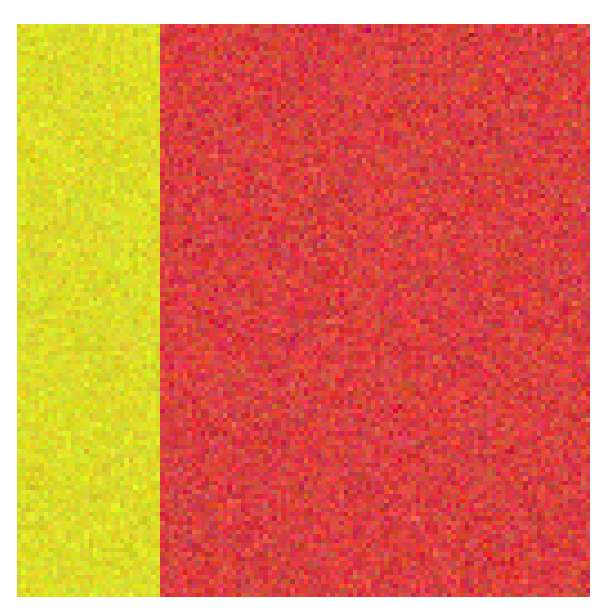
\includegraphics[width=1.75cm]{../images/syntheticexamples/X} } % Widest element
\newcommand{\sidecapX}[1]{ {\begin{sideways}\parbox{1.65cm}{\centering #1}\end{sideways}} }

\begin{figure}[ht]
\centering
\begin{tabular}{@{}c@{}}
\sidecapX{\scriptsize $X^0$} 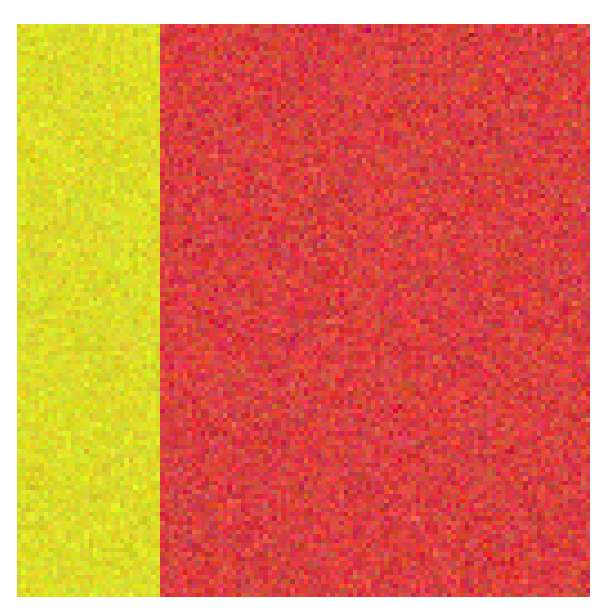
\includegraphics[width=.13\linewidth]{../images/syntheticexamples/X} \\
\sidecapX{\scriptsize $Y^0$} 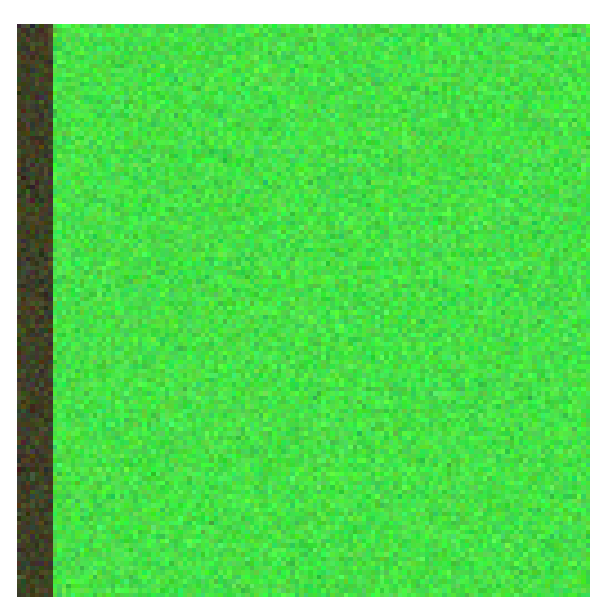
\includegraphics[width=.13\linewidth]{../images/syntheticexamples/Y} \\
\hspace{0.4cm} (a)\vspace{-0.25cm}
\end{tabular} 
\begin{tabular}{@{}c@{\hspace{1mm}}c@{\hspace{1mm}}c@{}}
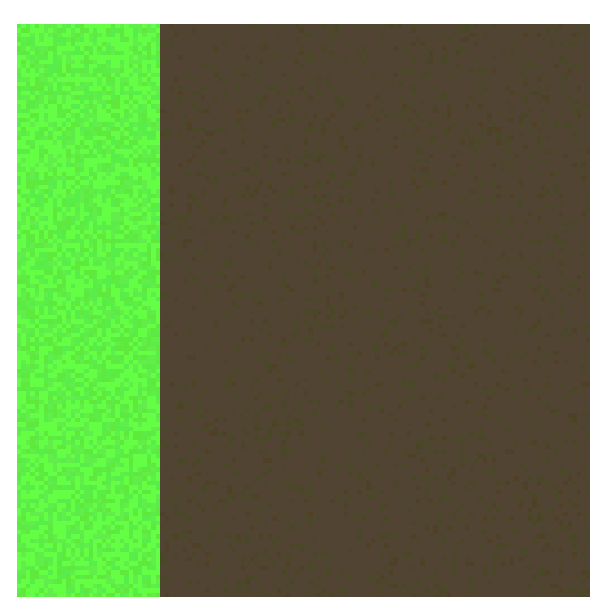
\includegraphics[width=.27\linewidth]{../images/syntheticexamples/symmetricsyntheticinv_l0_KX8_KY8_nn4} &
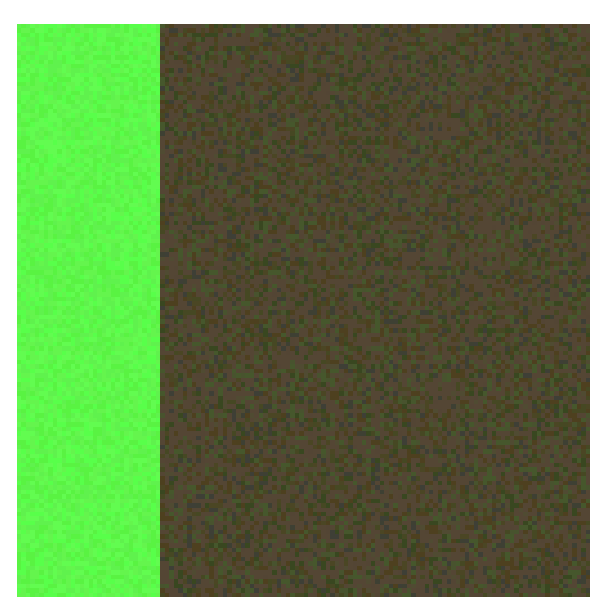
\includegraphics[width=.27\linewidth]{../images/syntheticexamples/symmetricsyntheticinv_l0001_KX8_KY8_nn4} &
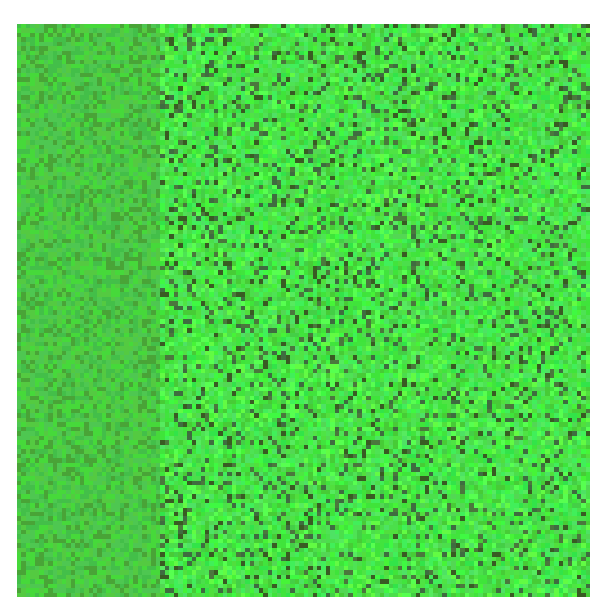
\includegraphics[width=.27\linewidth]{../images/syntheticexamples/symmetricsyntheticinv_l10_KX8_KY8_nn4} \\
(b) &  (c) & (d) \vspace{-0.25cm}
\end{tabular} 
\caption{Effect of changing the parameters $\la_X$ and $\la_Y$ of the relaxed and regularized OT formulation presented in section~\ref{sec:regsymme}, using parameters $\kappa=(0.1,8,0.1,8)$.  
	{(a)} original input images, 
	{(b)} relaxed OT, $\la_X=\la_Y=0$; 
	{(c)} $\la_X=\la_Y=0.001$; 
	{(d)} $\la_X=\la_Y=10$. 
	Each of these mappings can be observed in Figure~\ref{exlk}.\vspace{-0.1cm}}
  \label{im:synth}
\end{figure}

\paragraph{Number $N$ of quantization points}

In our numerical experiments, we have used $N=400$, which corresponds to a tradeoff between computation time and visual quality. In practice, of course, this number should be set as a function of the complexity (e.g. number of modes) of the input color distributions, but we found that $N=400$ was sufficient for all considered images in our tests.  Figure~\ref{changeN} shows some experiments to support this claim and to show that even setting $N$ to a smaller value did not affect the results much. 
 
 % For images with a small number of homogeneous regions, where we could do with less clusters, the points just cluster around a single value. Then, for images with a huge amount of regions, it seems that 400 is enough to summarize the information, of course this value may depend on the size of the image. 

 % Given the moderate impact of a change in this parameter, we decided to not introduce these experiments in the paper. 
 
\newcommand{\myfigb}[1]{\includegraphics[width=.25\linewidth,height=.25\linewidth]{./images/influence-quantiz/#1}}

\begin{figure}[h!]
\centering
\begin{tabular}{@{}c@{\hspace{1mm}}c@{\hspace{1mm}}c@{\hspace{1mm}}c@{}}
\myfigb{parrot_1.jpg} &
\myfigb{parrotX_N64} &
\myfigb{parrotX_N144} &
\myfigb{parrotX_N400} \\
\myfigb{parrot_2.jpg} &
\myfigb{parrotY_N64} &
\myfigb{parrotY_N144} &
\myfigb{parrotY_N400} \\
Original & $N=64$ & $N=144$ & $N=400$
\end{tabular}
\vspace{0.1in}
\begin{tabular}{@{}c@{\hspace{1mm}}c@{\hspace{1mm}}c@{\hspace{1mm}}c@{}}
\myfigb{flowers-1} & 
\myfigb{flowersX_N64} &
\myfigb{flowersX_N144} &
\myfigb{flowersX_N400} \\
\myfigb{flowers-2} & 
\myfigb{flowersY_N64} &
\myfigb{flowersY_N144} &
\myfigb{flowersY_N400} \\
Original & $N=64$ & $N=144$ & $N=400$\vspace{-0.1cm}
\end{tabular}
\caption{Results obtained computing the relaxed-regularized OT between the original images, changing the value of $N$. The parameters were set as $n=4$, $M=N$, for all experiments. Then, for the first and second row $\kappa=(0.1,1 ,0.1,1)$, and $\la_X=\la_Y=0.001$. For the second experiment that involves the third and forth row, $\kappa=(0.1,1.1 ,0.1,1.1)$ and $\la_X=\la_Y=9 \cdot 10^{-4}$. Each column corresponds to a single experiment which differ on the value of $N$.\vspace{-0.1cm}}

%\caption{Results obtained computing the relaxed-regularized OT between the image in the first and third row ($X$) with the image in the second and forth row ($Y$), respectively. The parameters were set as $n=4$, $M=N$, for all experiments. Then, for the first and second row $\kappa=(0.1,1 ,0.1,1)$, and $\la_X=\la_Y=0.001$. For the second experiment that involves the third and forth row, $\kappa=(0.1,1.1 ,0.1,1.1)$ and $\la_X=\la_Y=9 \cdot 10^{-4}$. Each column corresponds to a single experiment which differ on the value of $N$.\vspace{-0.1cm}}
\label{changeN}
\end{figure}


%%%%
\paragraph{Number $n$ of nearest neighbors} 

As for the other parameters of the method, the value of $n$ is set in order to obtain the best visual result.  This parameter is related to the connectivity of the graphs $\mathcal{G}_X$ and $\mathcal{G}_Y$. There are two behaviors that we need to avoid when setting it: 
\begin{itemize}
\item Too small $n$: The graph has very few edges. So, an area that is almost homogeneous in the spatial domain could end up being disconnected. In this case, this homogeneous area in the original image could be transported to different locations, generating color artifacts. In practice, this situation has been observed only for very small values of $n$. An example can be seen in  the first row of Figure~\ref{imn}, for $n=1$ and $n=2$ there is an area in the background that after the color matching gets two different colors. For greater values of $n$ this artifact disappears. 
\item Too large  $n$: The graph has a lot of edges and all the points are very interconnected, so the regularization term plays a very strong role by maintaining the structure of the graph in the original cloud of points, which reduces the flexibility of the map. This effect is quite difficult to observe in the resulting images. 
\end{itemize}
\newcommand{\myfig}[1]{\includegraphics[width=.25\linewidth]{./images/influence-nn/#1}}

\begin{figure}[h]
\centering
\begin{tabular}{@{}c@{\hspace{1mm}}c@{\hspace{1mm}}c@{\hspace{1mm}}c@{}}
\myfig{parrotX_nnx1} &
\myfig{parrotX_nnx2} &
\myfig{parrotX_nnx4} &
\myfig{parrotX_nnx10} \\
\myfig{parrotY_nnx1} &
\myfig{parrotY_nnx2} &
\myfig{parrotY_nnx4} &
\myfig{parrotY_nnx10} \\
\myfig{flowersX_nnx1} &
\myfig{flowersX_nnx2} &
\myfig{flowersX_nnx4} &
\myfig{flowersX_nnx10} \\
\myfig{flowersY_nnx1} &
\myfig{flowersY_nnx2} &
\myfig{flowersY_nnx4} &
\myfig{flowersY_nnx10} \\
$n=1$ & $n=2$ & $n=4$ & $n=10$
\end{tabular}
\caption{Results obtained by changing the $n$ parameter. The original images are presented in Fig.~\ref{changeN}}
\label{imn}
\end{figure}

As pointed out before, in our experiments we saw that setting $n=4$ avoids situations related to both cases. In Fig.~\ref{imn}, we can see how the final image evolves with a change in the value of the parameter $n$. Note that the only noticeable difference between the images can be observed on the results obtained with very small $n$ values ($n=1,2$) where homogeneous areas get divided. %Above a certain value, the results do not change.



%%%%


%%%%%%%%%%%%%%%%%%%%%%%%%%%%%%%%%%%%%%%%%%%%%%%
\subsection{Results}


Figure~\ref{star} shows some results on natural images and compare them with the methods of Piti\'e et al.~\cite{Pitie07}, Rabin et al.~\cite{Rabin_ip11}\footnote{We thank Julien Rabin for providing us these results} and Papadakis et. al~\cite{Papadakis_ip11}. Note that the method of~\cite{Pitie07} includes a post-processing step to reduce the color artifacts, but that it is applied here without the post-processing (it thus corresponds to the application of an approximate optimal transport).
 The goal of the experiment is to transfer the color palette of the images in the second row to the image on the first row.  Note that the methods in the state of the art introduce color artifacts (in the first column there is violet outside the flower, and in the second column the wheat is blueish), which can be avoided with the proposed method by an appropriate choice of $\la_X$, $\la_Y$ and $\kappa$. These results were obtained setting $N=400$ and constructing the graph as a $4$-nearest neighbor graph. By column, the values of $\la_X=\la_Y$ are $9\times 10^{-4}, 5\times 10^{-4}$, and $10^{-3}$ and $\kappa$ was set to (0.1,1.1,0.1,1.1), (0.1,1.3,0.1,1.3), and (0.1,1,0.1,1), respectively.
 

\newlength{\mylen}\settowidth{\mylen}{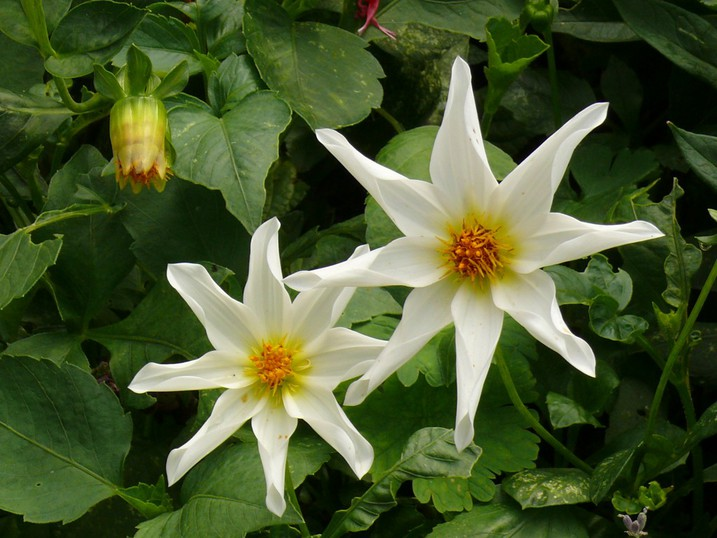
\includegraphics[width=3.8cm,height=3.3cm]{star/fleur_1}} % Widest element

\newcommand{\sidecap}[1]{{\begin{sideways}\parbox{3.3cm}{\centering #1}\end{sideways}} \hspace{-4mm}}

\newcommand{\myimg}[1]{\includegraphics[width=.25\linewidth,height=.22\linewidth]{#1}}


\begin{figure}[!ht]
\centering
\begin{tabular}{@{}@{}cc@{\hspace{1mm}}c@{\hspace{1mm}}c@{}}
\sidecap{ Original $X^0$ }  & 
\myimg{star/fleur_1} &
\myimg{star/wheat_1.jpg} &
\myimg{star/parrot_1.jpg} \vspace{-0.45cm}\\
\sidecap{ Original $Y^0$ } & 
\myimg{star/fleur_2} &
\myimg{star/wheat_2.jpg} &
\myimg{star/parrot_2.jpg}\vspace{-0.45cm} \\
\sidecap{ Piti\'e et al.~\cite{Pitie07} } & 
\myimg{star/fleur_pitie} &
\myimg{star/wheat_pitie} &
\myimg{star/parrot_pitie}\vspace{-0.45cm} \\
\sidecap{ Rabin et al.~\cite{Rabin_ip11} } & 
\myimg{star/fleur_Rabin} &
\myimg{star/wheat_Rabin} &
\myimg{star/parrot_Rabin}\vspace{-0.45cm} \\
\sidecap{ Papadakis et al.~\cite{Papadakis_ip11} } & 
\myimg{star/fleur_papadakis} &
\myimg{star/wheat_papadakis}  &
\myimg{star/parrot_papadakis} \vspace{-0.45cm}\\
\sidecap{ Proposed method } & 
\myimg{symmetric/symmetricfleur_l00009_KX11_KY11_nn4.eps} &
\myimg{symmetric/symmetricwheat_l00005_KX13_KY13_nn4.eps} &
\myimg{symmetric/symmetricparrot_l0001_KX1_KY1_nn4.eps} \\
 & (a) & (b) &(c)\vspace{-0.25cm}
\end{tabular}
\caption{Comparison between the results obtained with our method and with the methods of~\cite{Pitie07}, ~\cite{Rabin_ip11}  and~\cite{Papadakis_ip11} for image color transfer. Note how the proposed method is able to generate results without color artifacts for example, in \textbf{(a)} the violet color of the flower is not spread outside the flower, in \textbf{(b)} the wheat does not become bluish and in \textbf{(c)} the result does not enhance or colorize differently the flat areas of the background.\vspace{-0.25cm}}
\label{star}
\end{figure}

